\documentclass[tikz,border=2pt]{standalone}
\usepackage{amsmath}
\usepackage{pgfplots}
\pgfplotsset{compat=1.18}
\usetikzlibrary{arrows.meta}
\begin{document}
% Inventory level I (solid) and position P (dashed) under (s,S) = (3,9), lead time l = 2, I_1 = P_1 = 5,
% demands 2,4,3,1,2,2. Period k runs from k-1 to k: I_k = 5,3,-1,2,1,6, I'_k = 3,-1,-4,1,-1,4;
% P_k = 5,9,5,9,8,6, P'_k = 3,5,2,8,6,4. Orders Q_2 = 6 and Q_4 = 7 arrive at the starts of periods 4 and 6.
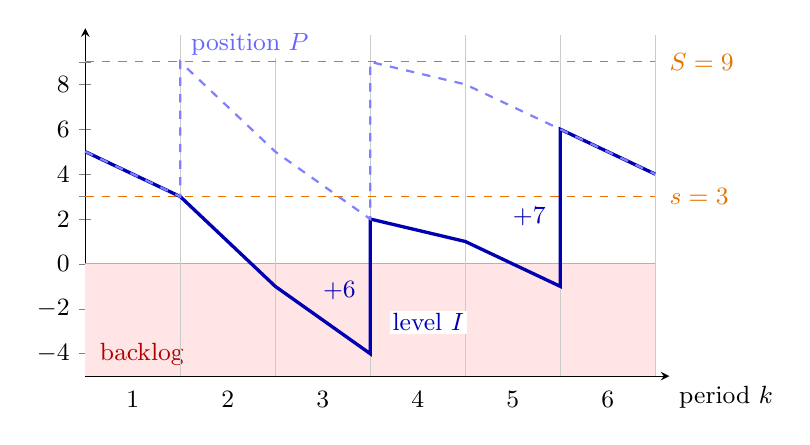
\begin{tikzpicture}[font=\small, >={Latex[length=2mm]}]
  \begin{axis}[
    axis lines=left, xmin=0, xmax=6.15, ymin=-5, ymax=10.5,
    xtick={0.5,1.5,2.5,3.5,4.5,5.5}, xticklabels={1,2,3,4,5,6}, xtick style={draw=none},
    ytick={-4,-2,0,2,4,6,8}, extra y ticks={3,9}, extra y tick labels={},
    xlabel={period $k$},
    xlabel style={at={(axis description cs:1,0)}, anchor=north west},
    width=9cm, height=6cm, clip=false
    ]
    \fill[red!10] (axis cs:0,-5) rectangle (axis cs:6,0);
    \node[red!70!black, anchor=south west] at (axis cs:0.05,-4.95) {backlog};
    \draw[gray!60, thin] (axis cs:0,0) -- (axis cs:6,0);
    \pgfplotsinvokeforeach{1,...,6}{\draw[gray!40, thin] (axis cs:#1,-5) -- (axis cs:#1,10.2);}
    \draw[orange!90!black, thin, dashed] (axis cs:0,3) -- (axis cs:6,3);
    \draw[orange!90!black, thin, dashed] (axis cs:0,9) -- (axis cs:6,9);
    \node[orange!90!black, anchor=west] at (axis cs:6.05,3) {$s=3$};
    \node[orange!90!black, anchor=west] at (axis cs:6.05,9) {$S=9$};
    % inventory level
    \addplot[blue!70!black, very thick] coordinates
      {(0,5) (1,3) (2,-1) (3,-4) (3,2) (4,1) (5,-1) (5,6) (6,4)};
    % inventory position
    \addplot[blue!50, thick, dashed] coordinates
      {(0,5) (1,3) (1,9) (2,5) (3,2) (3,9) (4,8) (5,6) (6,4)};
    \node[blue!70!black, anchor=west, fill=white, inner sep=1pt] at (axis cs:3.2,-2.6) {level $I$};
    \node[blue!60, anchor=south west, fill=white, inner sep=1pt] at (axis cs:1.08,9.15) {position $P$};
    \node[blue!70!black, anchor=east] at (axis cs:2.95,-1.2) {$+6$};
    \node[blue!70!black, anchor=east] at (axis cs:4.95,2.1) {$+7$};
  \end{axis}
\end{tikzpicture}
\end{document}
